% !TEX root = ../main_final_en.tex
% sections/03_literature_review.tex
\section{Literature Review}

The precise quantification of forest resources has historically been one of the cornerstones of territorial management and natural resource economics. The evolution of techniques for measuring tree growth and, more recently, for estimating biomass and carbon content, reflects a profound transformation in human society's priorities with respect to forest ecosystems. What began in medieval Europe as a logistical need to ensure the supply of firewood and structural timber in the face of scarcity has metamorphosed in the 21st century into a high-technology scientific discipline driven by global climate urgency \cite{brack_history_2000}.

Traditional dendrometry, the pillar of modern forest inventories, is based on the use of allometric relationships to estimate biomass ($w$) and other ecological parameters from easily measurable field variables, mainly diameter at breast height ($D$) and total height ($H$). These estimates are usually articulated through equations of the form:
\begin{equation}
    w = a D^b H^c
\end{equation}
or their logarithmic transformations:
\begin{equation}
    \lg w = a + b \lg D + c \lg H
\end{equation}
where parameters $a, b$ and $c$ are empirical regression coefficients \cite{shi2017methods}. In this context, the precision of primary measurements is critical, since, given the potential nature of these functions, errors in measuring $D$ and $H$ propagate and amplify in the final calculation of volume and carbon content. Despite the apparent simplicity of the fitting, results can be very good, as shown in Figure~\ref{fig:moso_bamboo}. However, there is a tension in the literature between the use of ``pantropical'' or generalised equations and species- or site-specific equations, since biases can be introduced if the architecture of local trees differs from the global one \cite{shang2025allometric}.

\begin{figure}
    \centering
    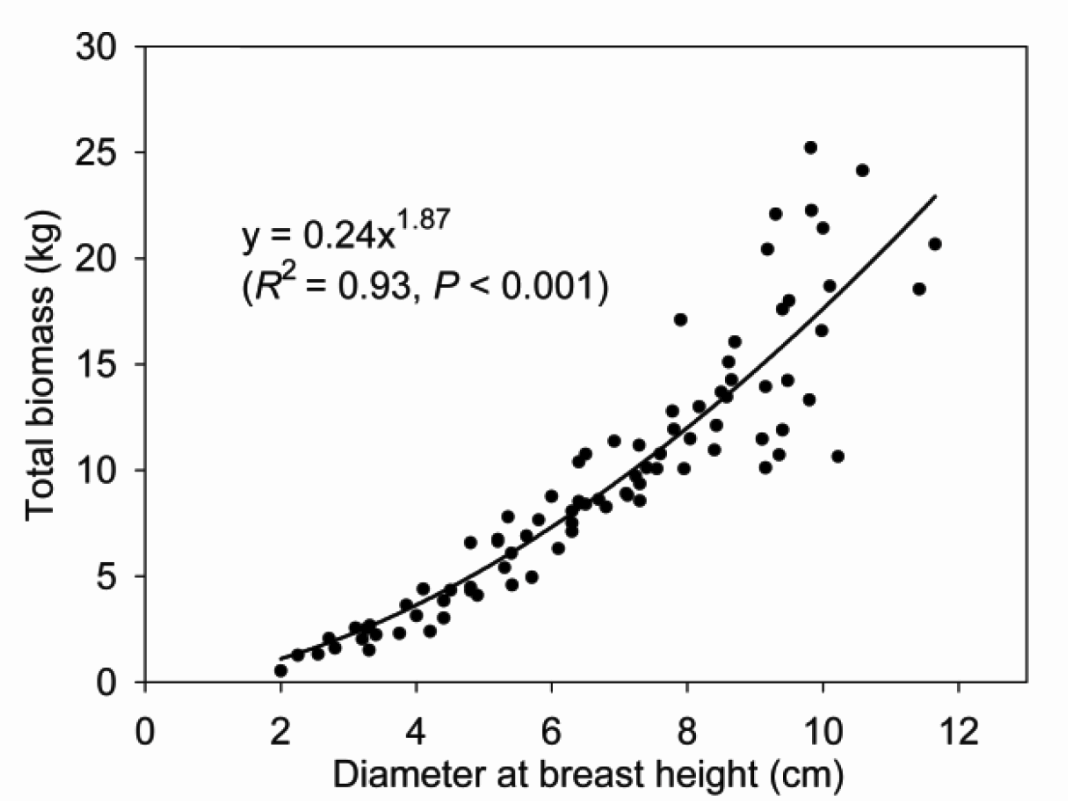
\includegraphics[width=\linewidth]{figuras/03_revision_literatura/moso_bamboo.png}
    \caption{Relationship between total biomass in kilograms and diameter at breast height in centimetres for moso bamboo \textit{(Phyllostachys edulis)}. Seen in \cite{shi2017methods}, with \cite{qi2016combining} as the original source.}
    \label{fig:moso_bamboo}
\end{figure}



The measurement of tree height has historically posed a greater challenge than that of diameter. Until the 1990s, mechanical hypsometers based on trigonometry predominated, which required manually measuring the distance to the tree and a clear line of sight \cite{nyakudanga_treemes}. These methods suffered from limitations of accuracy and ergonomics. The introduction of electronics marked a turning point by using ultrasound to measure distances automatically, enabling work in dense understoreys and improving precision to below 1\% \cite{nyakudanga_treemes}. At the same time, modern electronic callipers (an instrument measuring the linear distance between two parallel tangents to the tree stem) have digitised data collection, integrating measurement and metadata recording to minimise transcription errors \cite{nyakudanga_treemes}.

Subsequently, the introduction of laser scanning technology represented a revolution in forest measurement, overcoming the logistical and accuracy limitations of traditional methods. This technology is deployed mainly in two modalities: terrestrial laser scanning (TLS), which captures the three-dimensional structure of the forest from the ground with millimetre detail \cite{Kristiansen2018}, and airborne LiDAR. The latter is a method that uses light pulses to measure distances. Large-scale surveys typically consist of a LiDAR system mounted on an aircraft, helicopter, drone or satellite, which measures the distance to objects below it. One advantage is that, just as light can reach the ground through gaps in tree crowns, LiDAR laser pulses do so too, as we can observe in Figure~\ref{fig:lidar_avion}.
\begin{figure}
    \centering
    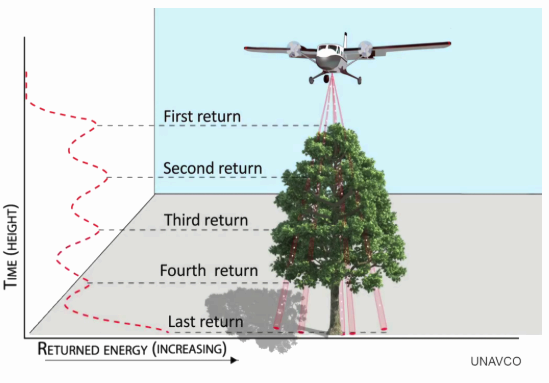
\includegraphics[width=\linewidth]{figuras/03_revision_literatura/lidar_avion.png}
    \caption{Diagram of a tree being scanned by an airborne LiDAR system and the various reflected pulses. Image obtained from \cite{opentopography_lidar_basics}.}
    \label{fig:lidar_avion}
\end{figure}
This means that in a single overflight various layers at different heights can be captured, enabling 3D reconstructions of the scanned area. The level of detail achievable is so high that individual trees can be identified, as seen in Figure~\ref{fig:chm_example}.


\begin{figure}
    \centering
    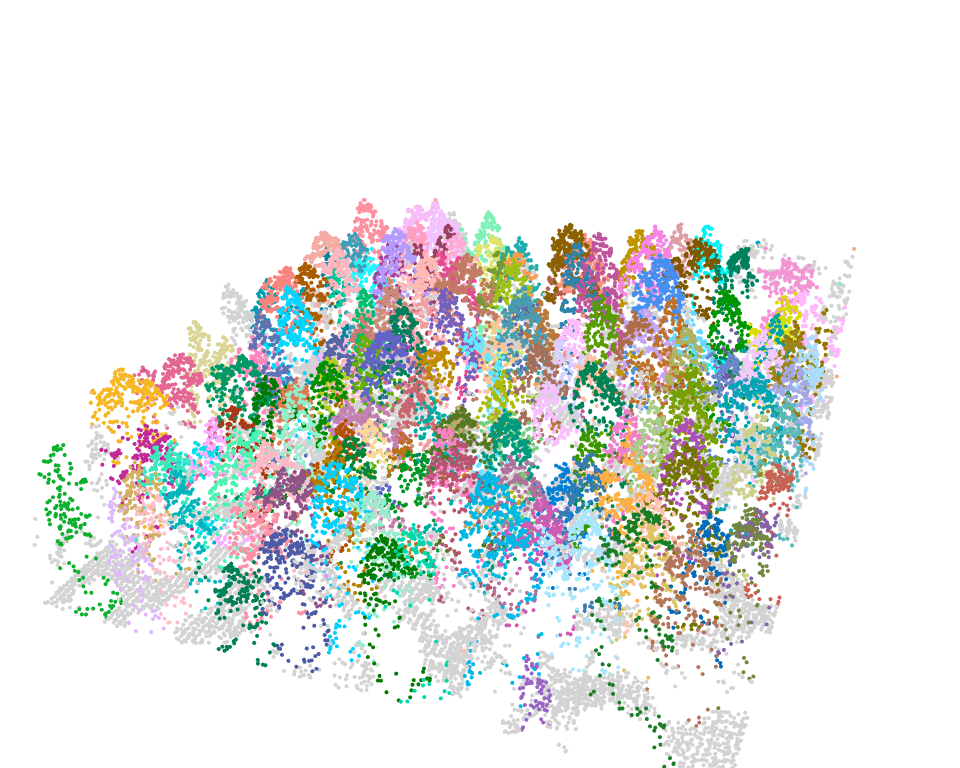
\includegraphics[width=\linewidth]{figuras/03_revision_literatura/CHM_1.png}
    \caption{Visualisation of a forest scanned with LiDAR. The possibilities of identifying individual trees in a dense forest environment are shown \cite{roussel2024lidrbook_itd}.}
    \label{fig:chm_example}
\end{figure}


% \begin{figure}
%     \centering
%     \begin{subfigure}[b]{0.48\linewidth}
%     \centering
%     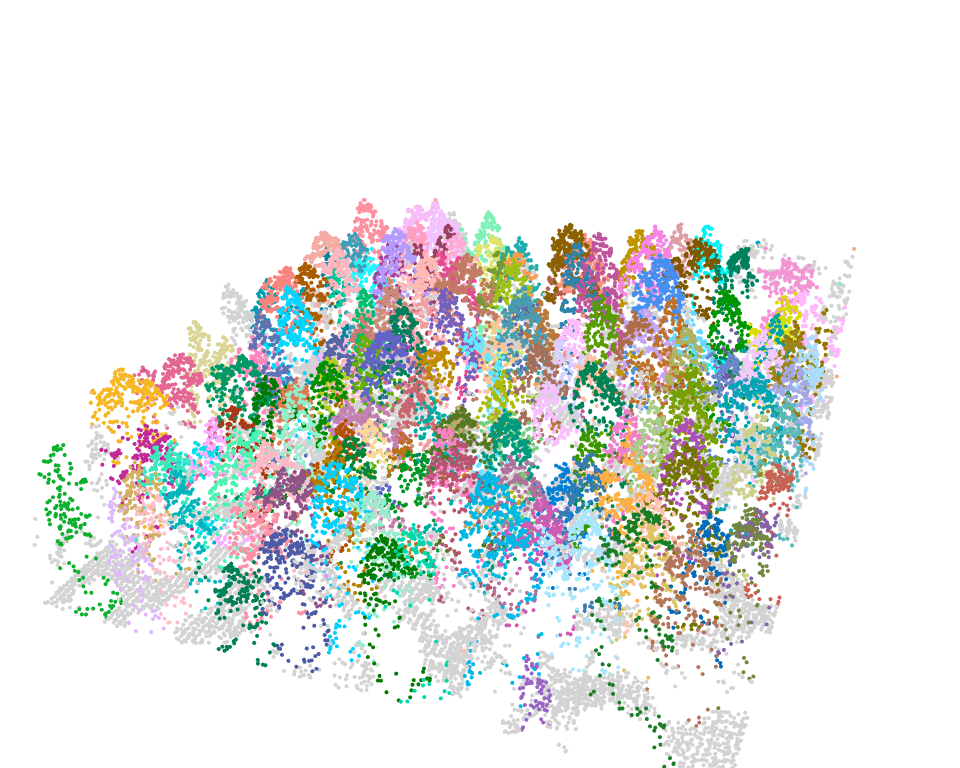
\includegraphics[width=\linewidth]{figuras/03_revision_literatura/CHM_1.png}
%     \caption{3D visualisation of a forest scanned with LiDAR. Each tree has been identified with a different colour.}
%     \label{fig:lit_sub1}
%     \end{subfigure}
%     \hfill
%     \begin{subfigure}[b]{0.48\linewidth}
%         \centering
%         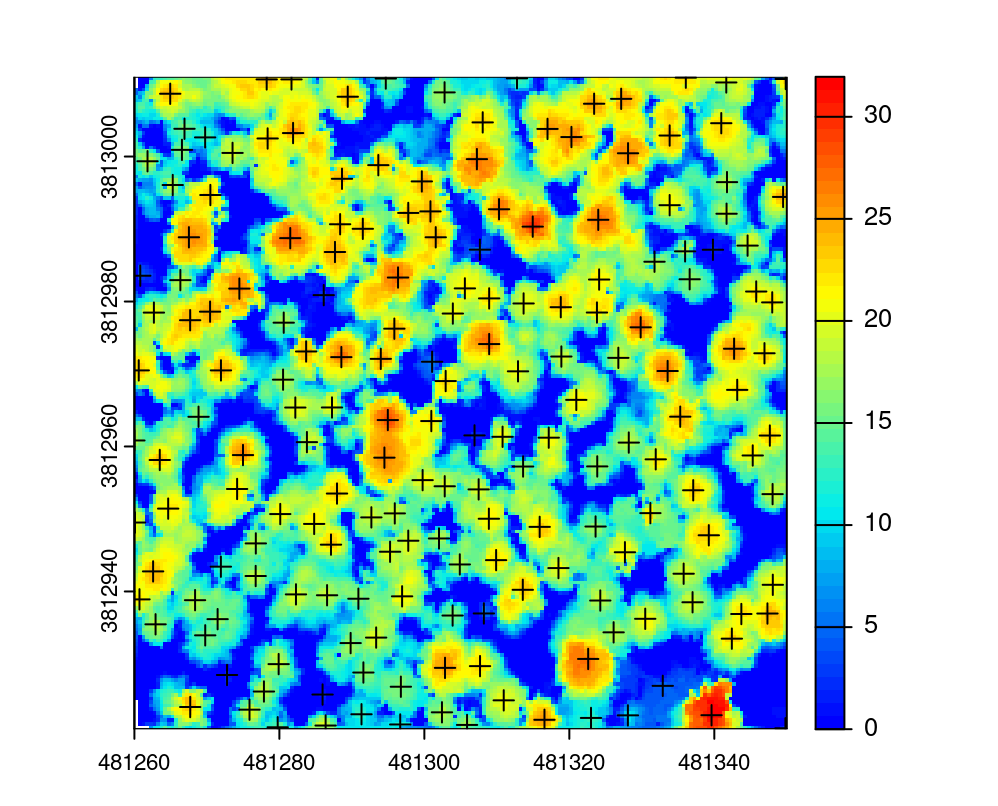
\includegraphics[width=\linewidth]{figuras/03_revision_literatura/CHM_2.png}
%         \caption{Same mapping but seen from above as a 2D map. Each tree is marked with an \textbf{x}.}
%         \label{fig:lit_sub2}
%     \end{subfigure}
%     \caption{Visualisation of a forest scanned with LiDAR. The possibilities of identifying individual trees in a dense forest environment are shown.}
%     \label{fig:chm_example}
% \end{figure}

The main limitations of airborne LiDAR lie in its high cost and logistical complexity. These factors hinder large-scale coverage with optimal periodicity, also generating significant latency in the availability of regional data. Furthermore, processing this information is more demanding than previous methods, compounded by the technical challenge of managing and storing large volumes of data. Figure~\ref{fig:pnoa_lidar} shows the data acquisition plan for the Third cycle of the PNOA-LiDAR project of Spain's National Geographic Institute, where the cadence of mappings can be appreciated.

\begin{figure}
    \centering
    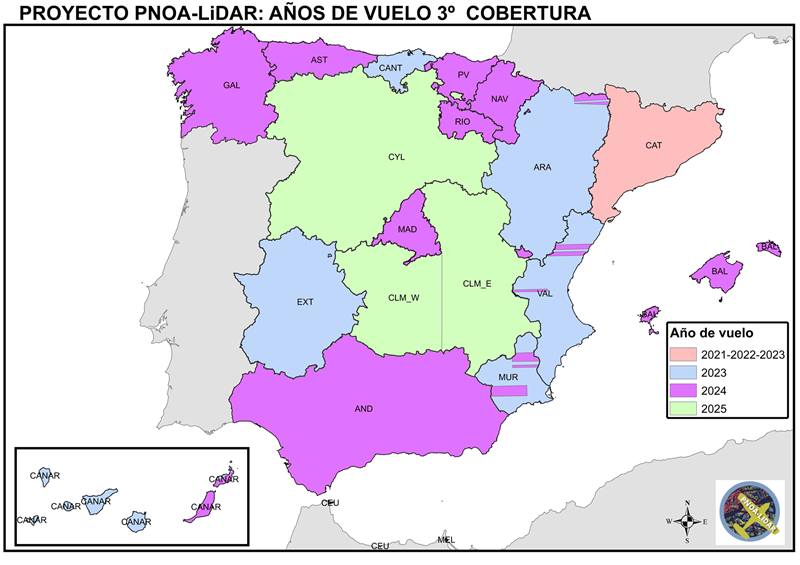
\includegraphics[width=\linewidth]{figuras/03_revision_literatura/plan_lidar_mapeo.png}
    \caption{Data acquisition plan for the Third cycle of the PNOA-LiDAR project of Spain's National Geographic Institute \cite{ign_pnoa_lidar_tercera}.}
    \label{fig:pnoa_lidar}
\end{figure}


The integration of these structural data, together with satellite remote sensing and the large-volume data processing capability offered by machine learning algorithms, has inaugurated a new paradigm: the ability to monitor forest resources at global scale with unprecedented precision. It is in this context of ``precision forestry'' and large-scale Earth observation that current research is situated, with very promising results having been achieved that enable the complexity of forest ecosystems to be addressed with a granularity previously unattainable.


